\documentclass[class=minimal, border = 0pt, crop]{standalone}
\usepackage{pgf}
\usepackage{tikz}
\usepackage[utf8]{inputenc}
\usetikzlibrary{arrows,automata,shapes,calc, backgrounds}
\usetikzlibrary{positioning}
\pagestyle{empty}
\tikzset{
    state/.style={
           rectangle,
           rounded corners,
           draw=black, very thick,
           minimum height=2em,
           inner sep=5pt,
           text centered,
           },
    pil/.style={
           ->,
           thick,
           shorten <=4pt,
           shorten >=4pt,
           },
    ball/.style={
           circle,
           draw,
           align=center,
           anchor=north,
           inner sep=0,
           fill=black,
           }
}

\begin{document}
\centering
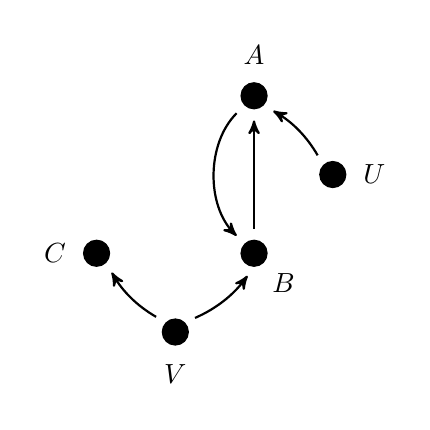
\begin{tikzpicture}[->,>=stealth']
\tikzstyle{every node}=[draw,shape=circle, fill=black]
\node (a1) at (0,0) [label=above:$A$] {};
\node (a2) at (0,-2) [label=south east:$B$] {};
\node (a3) at (1,-1) [label=right:$U$] {};
\node (a4) at (-2,-2) [label=left:$C$] {};
\node (a5) at (-1,-3) [label=below:$V$] {};
\path (a2) edge[pil] (a1);
\path (a1.south west) edge[pil, bend right = 45] (a2.north west);
\path (a3.north west) edge[pil, bend right = 15] (a1.south east);
\phantom{\path (a4) edge[pil] (a2);}
\phantom{\path (a3.south west) edge[pil, bend left = 15] (a2.north east);}
\path (a5.north west) edge[pil, bend left = 15] (a4.south east);
\path (a5.north east) edge[pil,color = black, bend right = 15] (a2.south);
\end{tikzpicture}
\end{document}